
\documentclass[12pt]{article}
\usepackage{verbatim}
\usepackage{cite}
\usepackage{graphicx}

\bibliographystyle{abbrv}

\begin{document}

\title{P2 Dataflow Architecture}
\author{}

\date{}
\maketitle
\newcommand{\eat}[1]{}

\section{Introduction}

This document provides an overview of the P2 dataflow architecture.
The focus of this document is on the new P2 Dataflow Language (P2DL), put in place
for quickly building dataflow graphs out of P2 'Element' objects. The language 
syntax resembles much of the Click dataflow language~\cite{click-tocs} with some 
added support for runtime dataflow edits. Some familiarity with P2 elements is a
requirement to understanding this document. Section~\ref{sec:basic} provides
an overview of the basic P2 dataflow architecture and can be skipped for those already
familiar with P2.

The P2DL compiler is written in Yapps v2 grammar and requires the P2 python 
library extensions.  % JJJ: (section 3)
Support for compiling a P2DL description from C++ is provided by a DataflowInstaller
P2 element. P2DL defines a declarative interface to specify the vertices and edges 
of a P2 dataflow graph. A vertex in the dataflow graph description is a P2 element, 
and an edge specifies how two elements
should be connected. The P2DL compiler takes a dataflow description and produces
a Plumber::Dataflow (or a Plumber::DataflowEdit in the case of an edit) object that 
can be installed into a running P2 Plumber. The P2 Plumber installs the dataflow 
or the edit if it is valid. The installation of a dataflow or edit that is not valid will not
affect the dataflows of a running system.  

This document describes the new P2 Dataflow Language (P2DL) and incremental OverLog rule installer,
as well as a description of the relevant aspects of the P2 architecture. In section~\ref{sec:basic}, 
we provide a brief overview of P2 elements and how these elements are connected to form a dataflow 
graph. Section~\ref{sec:python} describes the P2 Python library, which was used to build the P2DL 
compiler. The remainder of this document describes our main contribution --
a detailed description of the basic P2DL (Section~\ref{sec:p2dl}) language and the incremental 
OverLog rule installer (Section~\ref{sec:inc_install}).

\section{P2 Architecture}
\label{sec:basic}

\subsection{Overview}
This section describes the basic P2 dataflow architecture, shown in
Figure~\ref{fig:arch}, consisting of three primary components -- Plumber, 
Dataflow, and Element. An \emph{Element} defines a set of input and output 
ports for receiving and sending data. A set of
Elements form a \emph{Dataflow} by connecting output ports to the inputs ports
in some fashion. A Dataflow is then semantically checked and installed into a
\emph{Plumber}, which manages a set of Dataflows that share a single scheduler.
The remainder of this section explores each of these components in greater detail.
But first we must describe the basic data types that Elements use to process data
flowing through the system.

\begin{figure*}[htbp] %  figure placement: here, top, bottom, or page
   \centering
   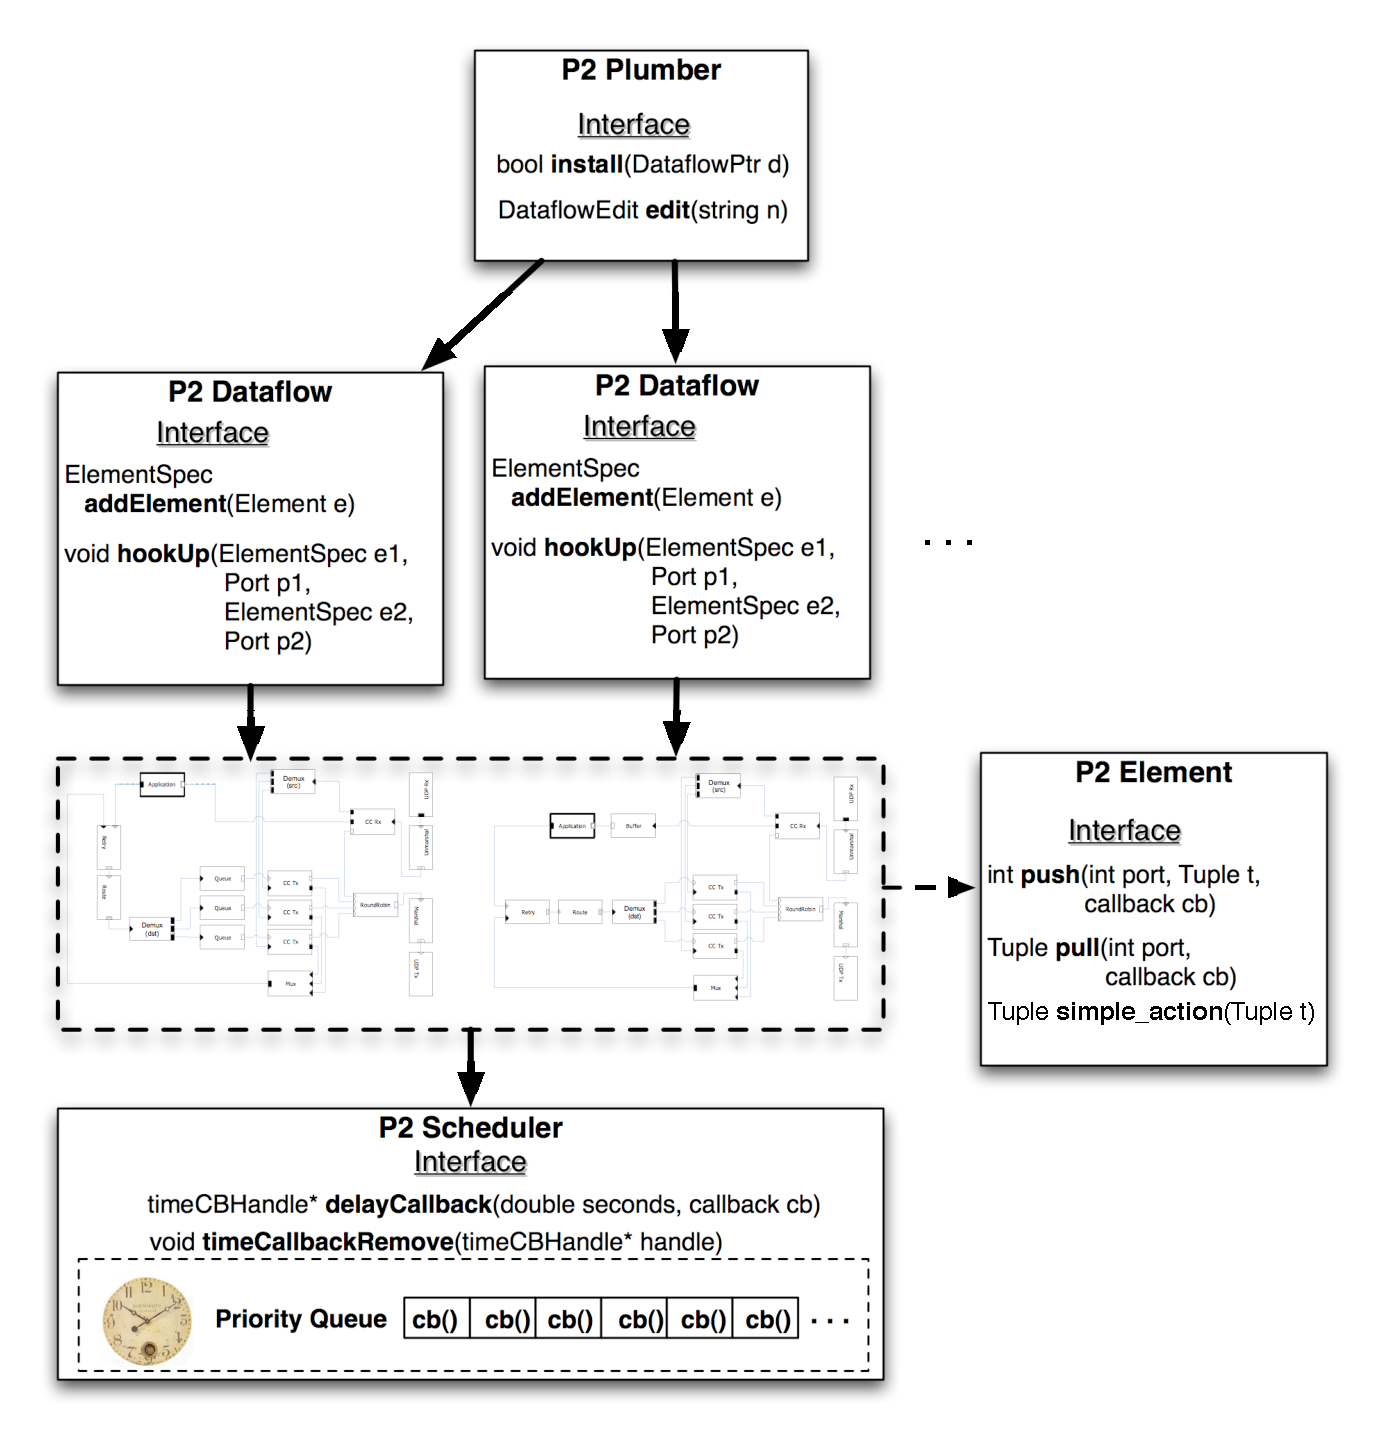
\includegraphics[width=4in]{dataflow_arch.eps} 
   \caption{Basic P2 dataflow architecture.}
   \label{fig:arch}
\end{figure*}


\subsection{P2 Data}
A \emph{tuple} (tuple.h) represents the data type that is passed between Elements in a 
Dataflow. A tuple contains a list of \emph{value} (value.h) types, which are defined
in the 'p2core' system directory and have a file name prefix='Val\_'. The types defined
include all the base C++ types (e.g., int, float, strings) as well as some non traditional
types (e.g., identity, lists, ip address, etc.). A tuple is an immutable object in the sense
that once an Element creates, it cannot be changed by some other Element in the
dataflow~\footnote{It can however be replaced with a completely new tuple created by
some downstream Element.}. 

\subsection{Element}
Each element defines a set of input ports and output ports.
Elements process the tuples that arrive on its input ports and send, possibly
new, tuples on its output ports. The kind of processing that is performed on a tuple
is specific to the Element type and possibly the port on which a tuple is received. 
There are three types of ports that an Element can define on its interface, and 
depending on the interface (input or output) these port types have different semantics.
The following enumerates the semantics of each possible port type.
\begin{enumerate}
\item A \emph{push input} port means that data will be "pushed" to the Element in a
\emph{function call} like fashion. 
\item A \emph{pull input} port means that the Element itself will "pull" from the upstream Element when it is ready to receive the next tuple.
\item A \emph{push output} port means that the Element will call ("push") the
downstream Element when it has generated a new tuple.
\item A \emph{pull output} port means that the downstream Element will call the Element
(defining the port) when it is ready to accept another tuple. 
\item A \emph{agnostic input/output} port means that both push and pull semantics 
are supported on the given Element port.
\end{enumerate}
Further details on defining Element ports can be viewed in element.h, located in 
the 'p2core' system directory. 

\begin{verbatim}
class Element {
    . . .
  virtual int push(int port, TuplePtr, b_cbv cb);

  virtual TuplePtr pull(int port, b_cbv cb);

  virtual TuplePtr simple_action(TuplePtr p);
    . . .
}
\end{verbatim}

Every Element defines three methods for receiving tuples, as shown above.
The actual methods that are called on receipt of a tuple depend on the port 
type. For all port types, the \emph{simple\_action} method will be called. An
Element that defines an agnostic port will likely make use of this method.
A push input port will call the \emph{push} method of the Element receiving the
tuple. The tuple is passed as an argument in the push method. A pull output will 
call the \emph{pull} method of the Element being requested and the Element 
will return the tuple.

In some cases the element receiving the tuple, via either a push or pull port, is no
longer willing to accept further tuples. For this reason, both push and pull methods 
take a callback method formal of type \emph{b\_cbv} having the following signature.
\begin{verbatim}
    typedef boost::function<void (void)> b_cbv;
\end{verbatim}
The above type refers to a boost function with \emph{void} formals and returning
\emph{void}. When an upstream Element issues a push to a downstream Element, 
that can accept no further tuples, the downstream element will register the 
upstream Element's callback and return $0$. When a downstream Element issues
a pull to an upstream Element, that can produce no further tuples, the upstream element
will register the downstream Element's callback and return an empty tuple pointer.
The callback is defined by the calling Element and is used to signal
the Element when the counterpart (upstream or downstream) Element is ready to 
accept or produce more tuples. This mechanism permits flow control between 
Elements in the Dataflow, and is the primary difference between P2 and Click-like
Dataflows. 

\subsection{Dataflow}

A Dataflow is a collection of Elements whose ports have been completely connected 
to form a graph with Elements at the vertices and port connections as the edges. 
Tuples flow through the Dataflow as they are passed along the Element ports. 
Two Elements can be connected together if they have compatible ports. An output port is 
compatible with an input port if they are the same type (e.g., push, pull, or agnostic) or
at least one of the ports is agnostic. Before a Dataflow can be installed its ports are
semantically checked for type compatibility. Moreover, all agnostic ports in the 
Dataflow must resolve to either a push or a pull port. If there exists any port 
incompatibilities or some agnostic port(s) does not resolve the installation will fail.

\begin{verbatim}
class Plumber {
    class Dataflow {
        . . .
        virtual ElementSpecPtr addElement(ElementPtr);

        virtual void hookUp(ElementSpecPtr src, int src_port,
                            ElementSpecPtr dst, int dst_port );
         . . .
     }
 }
\end{verbatim}

The above class definitions show the relevant methods for adding Elements and
connecting Element ports in a Dataflow. The \emph{addElement} takes an initialized
\emph{ElementPtr} as argument and returns an \emph{ElementSpecPtr} to the caller. 
The caller uses all the \emph{ElementSpecPtr} objects returned by the 
\emph{addElement} method as arguments to the \emph{hookUp} method for 
connecting the output port of the \emph{src} formal to the input port of the 
\emph{dest} formal. The port numbers are indicated by the \emph{src\_port} and
the \emph{dst\_port} formals.

\pagebreak
\subsection{Plumber}
\begin{verbatim}
class Plumber {
        . . .
        int install(DataflowPtr d);
        . . .
 }
\end{verbatim}
A Plumber maintains a set of Dataflows that share a single scheduler. 
A Dataflow is installed into the the system through the \emph{install} method
defined by the \emph{Plumber}, which takes a DataflowPtr object as argument.
The installation checks the Dataflow for semantic correctness and ensures that
all ports have been assigned a counterpart. If any of these checks fail the 
\emph{install} method return a $-1$ value, and does not register the Dataflow.
If the Dataflow passes all checks a $0$ value is returned and the Dataflow is
finalized, during which all the Element \emph{initialize} methods are called.

\subsection{DataflowEdit}
\begin{verbatim}
class Plumber {
        . . .
        class DataflowEdit : public Dataflow {
            . . .
            ElementSpecPtr find(string);
            . . .
        }
        DataflowEditPtr new_dataflow_edit(string name);
        . . .
}
\end{verbatim}
A Dataflow that has been installed will be registered by the Plumber under the
Dataflow name. Thereby, permitting future edits to the Dataflow by calling the
{\bf new\_dataflow\_edit} method while passing the Dataflow name as 
argument. The return value of this method is a DataflowEditPtr, which defines
all the methods of the Dataflow class (for adding and connecting new Elements
to the Dataflow) as well as retrieving existing elements from the Dataflow using
the {\bf find} method of the DataflowEdit class. The {\bf find} method
returns an \emph{ElementSpecPtr} that can be used to rewire the existing Element
in whatever fashion you deem fit. Existing Elements that are completely 
disconnected from the Dataflow (by rewiring of the ports) through the edit will be 
garbage collected. Please see plumber.h for further details regarding the Plumber,
Dataflow, and DataflowEdit class structures. 

\section{P2 Python Library}
\label{sec:python}

The primary purpose of the P2 Python library extensions is to incorporate 
the basic Element and Dataflow structures into the Python runtime library. Doing so
enables Element and Dataflow operations in a Python environment. In particular,
the Python programmer can add Elements and hook them together to form a 
Dataflow using a Python script. The script can then install the Dataflow into a
running Plumber instance, after which all Element interactions execute entirely in 
C++. 

The Python module extensions permit the ability to incorporate C/C++ code
into a Python environment. The raw interface to the Python module extension library is
rather terse and for this reason we have made use of the Boost Python C++ 
library (http://www.boost.org/libs/python). Boost Python provides a set of C++ 
templates that allow for seamless interoperability between C++ and the Python
programming language. The rest of this section provides a complete description
of how we incorporate various P2 structures into Python using Boost.Python. The
Boost.Python website contains a tutorial that should be read in order to better 
understand the rest of this document.

\subsection{Library Organization}

The P2 Python library is housed in the '/python/p2' subdirectory. The 'p2python.cpp'
file contains the code that packages up all library extensions into a Python module
titled 'libp2python' that can be imported into the Python interpreter. Please refer
to the README file in 'python/p2' for details regarding compiling and environment
setup. The directory structure in 'python/p2' models the top level P2 directory 
structure. Each subdirectory contains a number of C++ files containing code that
imports, into the Python module, each P2 type within the respective top 
level directory. The next section provides more details on importing various P2
data structures.


\subsection{Importing P2 Data Structures}

\begin{verbatim}
  class_<Print, bases<Element>, boost::shared_ptr<Print>, boost::noncopyable>
        ("Print", init<std::string>())
    .def(init<std::string, int>())
    .def("class_name", &Print::class_name)
    .def("processing", &Print::processing)
    .def("flow_code",  &Print::flow_code)
  ;
\end{verbatim}

The Boost.Python library provides a template for generating the necessary code
that imports a C++ class. The template is titled 'class\_' and an example import
of the \emph{Print} Element can be seen above. The first argument to the template
is a reference to the C++ class definition. This is followed the class definitions, wrapped
in the {\bf bases} template, of the C++ classes that \emph{Print} inherits from, in this 
case the \emph{Element} class. The third argument specifies the reference type that
will hold the object after creation. Here we specify that a newly created \emph{Print}
object should be stored in a \emph{boost::shared\_ptr} type. The copy constructor
of the \emph{Element} class is private, so we need to indicate this by the fourth 
argument \emph{boost::noncopyable}. The template constructor follows the template
definition, and indicates the string name of the class (i.e., "Print") and the signature of
a constructor of the class wrapped using the \emph{init} template, which takes the
formal types of the constructor in the order they appear in the C++ class definition. 
Further constructor definitions can be added using the \emph{.def} macro, described
next. 

The \emph{class\_} template provides a \emph{.def} macro for importing some subset
of public methods in the C++ class definition. The first instance of the \emph{.def} 
macro in the above example defines another constructor to the \emph{Print} Element
that takes the indicated formal argument types. This is followed by the definition of
three instance methods that take the string method name as the first argument and
a pointer to the method within the class definition. 

\begin{verbatim}
  class_<Val_Str, bases<Value>, boost::shared_ptr<Val_Str> >
        ("Val_Str", no_init)
    .def("mk",  &Val_Str::mk)
    .staticmethod("mk")
  ;
\end{verbatim}

The definition above uses the \emph{class\_} template for importing the \emph{Val\_Str}
class. There are two differences, from the previous example, that are exhibited by this
example. The first comes from the fact that a P2 value does not define a constructor,
which is indicated by the {\bf no\_init} reference in place of the constructor definition.
The second is the definition of the static method {\bf mk}, which is defined using the
\emph{.def} macro along with a \emph{.staticmethod} macro call that takes the
string name of the static method as argument. Creating a \emph{Val\_Str} object
in Python will occur the same way as is done in C++ -- by calling the {\bf mk} method.

The P2 Python library uses Boost.Python to incorporate into Python data types such
as \emph{Dataflow}, \emph{Plumber}, \emph{Tuple}, \emph{Table}, 
\emph{Iterator}, and C++ vectors of \emph{Value} types. If you are programming a
new Element class and wish to incorporate that element into Python you must follow
these steps.
\begin{itemize}
\item Use the \emph{class\_} template to generate the Python definition of your new Element.
\item The \emph{class\_} definition of your new Element should be placed in 
a function definition, that takes void and returns void, and is defined in the respective 
'python/p2' subdirectory in a suitably named '.cpp' file.
\item Add your '.cpp' file to the {\bf Makefile.am} file within the chosen 'python/p2' 
subdirectory.
\item Add your function prototype to the 'python/p2/p2python.cpp' file and call the
function from within the {\bf BOOST\_PYTHON\_MODULE(libp2python)} block
expression.
\end{itemize}
There are many examples within the 'python/p2' directory of adding P2 Elements 
to the Python module in the above fashion. The next section describes how to use
the P2 Python module in a Python environment.

\subsection{P2 Python Programming}

The 'libp2python.so' shared object is created after successfully compiling the 
'python' directory structure. This shared object is what the Python interpreter loads
when importing the P2 module. The P2 module contains all the data structures
defined in the 'python/p2' subdirectories using the \emph{class\_} template. The
following is an example python session that creates a \emph{Plumber} and installs
 a \emph{Dataflow} containing two Elements.
 
\begin{verbatim}
Python 2.3.4 (#1, Feb  2 2005, 12:11:53) 
[GCC 3.4.2 20041017 (Red Hat 3.4.2-6.fc3)] on linux2
Type "help", "copyright", "credits" or "license" for more information.
>>> import libp2python # Import the P2 module
>>>  libp2python.eventLoopInitialize() # Initialize the event loop
>>> plumber = libp2python.Plumber()
>>> dataflow = libp2python.Dataflow("test")
>>> timed = dataflow.addElement(libp2python.TimedPushSource("timed", 0))
>>> discard = dataflow.addElement(libp2python.Discard("discard"))
>>> dataflow.hookUp(timed, 0, discard, 0)
>>> plumber.install(dataflow)
0
>>> libp2python.eventLoop() # Run the event loop
\end{verbatim}

The thing to note in the above example is that the method names and arguments
follow the respective C++ class definitions. Once a \emph{Dataflow} has been installed
into the \emph{Plumber} you can run it by calling the {\bf eventLoop} routine as shown
in the above example. The ability to create and install arbitrary Dataflow instances
allows one to encode the logic that determines the Element connections in the
Python Programming language. The new P2 Dataflow Language is one example 
Python program that compiles a high level dataflow language into calls that create
a \emph{Dataflow} instance in accordance to the language specification.

\subsubsection{Defining P2 Elements in Python}

This section assumes you have access to the 'python/p2/p2core/element.cpp' code
file, found in the P2 system directory. Given the ability to code the logic that creates,
installs, and runs a \emph{Dataflow} instance the P2 programmer need only write C++ 
code to create or modify P2 Element and Value types. Another option allowed by the P2 
Python library is to write a P2 Element as a Python class, which is the topic of this 
section. 

The \emph{Element} class is defined differently in the P2 Python module to 
allow for the definition of \emph{Element} classes in Python. The 'element.cpp' file 
contains the C++ \emph{Element} Python definition. However, instead of inheriting directory from the \emph{Element} class, the \emph{class\_} template inherits
from the \emph{ElementWrap} class definition (also defined in 'element.cpp'). The
\emph{ElementWrap} C++ class overrides the methods of the \emph{Element} class
in order to provide a dynamic dispatch to the respective overridden methods in
the Python class instance. That is, a Python class that inherits from the 
\emph{Element} class will actually inherit from the \emph{ElementWrap} class, which
automatically invokes any methods that the Python class overrides. Since the C++ 
compiler is unaware of the Python class definition, it will call the 
overridden methods of the \emph{ElementWrap} class, which will in turn invoke the 
Python interpreter to call the respective overridden Python method. If the Python class 
doesn't override a particular method then the \emph{ElementWrap} class will invoke 
the method defined in the parent \emph{Element} class.

The only known limitation of Boost.Python is the ability to pass a function from
Python to C++, and have that function be called from within C++. Given that callbacks
are an intricate part of \emph{Element} code, the \emph{ElementWrap} class defines
a few extra methods that the Python \emph{Element} programmer can use. The
following list the of methods or provided by the \emph{ElementWrap} class definition.
\begin{description}
\item [TuplePtr py\_pull(int port, object callback)] -- Calls {\bf pull} on the upstream element on the given port. If the upstream \emph{Element} blocks further calls a dispatch will be issued on the passed in callback method when further tuples can be pulled.
\item [int py\_push(int port, TuplePtr tp, object callback)] -- Calls the {\bf push} method of the downstream element on the given port. If the downstream element blocks further calls a dispatch is issued on the passed in callback method when further tuples can be pushed.
\item [timeCBHandle* set\_delay(double secondDelay, object callback)] -- Calls the {\bf delayCB} method. When the secondDelay expires a dispatch will occur to the Python method specified passed to the callback formal. A \emph{timeCBHandle*} object is produced, which can be used to cancel the timer using the {\bf cancel\_delay} method (described below). 
\item [void cancel\_delay(timeCBHandle*)] -- Cancels the outstanding delayed callback.
\end{description}
Other methods exist in \emph{ElementWrap} to provide the dynamic dispatch 
capability needed to call from C++ back into Python. The {\bf callback} formal
in the above methods specifies the method, defined in your Python class, that
is to be called by the dispatch method of the \emph{ElementWrap} class. The dispatch
method will not provide arguments to the Python method at call time. If your callback
requires the use of arguments then you should use wrap it inside of a Python lambda function
that will pass it the required arguments at call time.

\subsubsection{Example P2 Element class in Python}
\label{sec:element_example}

\begin{verbatim}
class Terminal(Element):
  def __init__(self, name):
      Element.__init__(self, name, 1, 1)
      self.self(self) # Pass the ElementWrap class a reference to the self object.
  def class_name(self): return "Terminal"
  def processing(self): return "h/h"
  def flow_code(self):  return "-/-"
  def initialize(self):
      self.timer = self.set_delay(0, self.delay_callback)
      return 0
  def callback(self, port):
      self.timer = self.set_delay(0, self.delay_callback)
  def delay_callback(self):
      # Read string from terminal and send 
      # it in a tuple to push output port 0.
      line = raw_input("P2 Terminal >> ")
      t = Tuple.mk()
      t.append(Val_Str.mk("terminal"))
      t.append(Val_Str.mk(text))
      t.freeze()
      if self.py_push(0, t, self.callback) > 0:
        self.timer = self.set_delay(1, self.delay_callback)
  def push(self, port, tp, cb):
      # Received some tuple on input port 0
      return 0
\end{verbatim}

The above \emph{Terminal} class is written entirely in Python and can be linked
into a P2 \emph{Dataflow} instance. The class overrides the {\bf initialize} method
to set a delayed callback using the {\bf set\_delay} method defined in the 
\emph{ElementWrap} class. The timeCBHandle is stored in the self.timer variable, which
can be used to cancel the timer using the {\bf cancel\_delay} method. 
When the P2 event loop calls the callback associated
with this timer it will invoke the {\bf ElementWrap::dispatch} method, which will
in turn invoke the {\bf delay\_callback} method defined by the Python \emph{Terminal}
instance. The {\bf delay\_callback} method in the \emph{Terminal} class definition
reads a line from {\bf stdin}, creates a tuple containing the text, and sends the tuple
to its output port $0$ using the {\bf py\_push} method provided by the 
\emph{ElementWrap} class. The {\bf ElementWrap::py\_push} method invokes pushes
the tuple to the output port $0$, which passes the {\bf callback} method as
the callback function argument. The remaining code in this Python class definition 
should be self explanatory.

\section{P2 Dataflow Language (P2DL)}
\label{sec:p2dl}

A P2DL description defines a set of P2 elements and specifies how those elements
should be hooked up to form a dataflow graph. The language specifies two types
of dataflow specifications, which are named {\bf dataflow} and {\bf edit}. A dataflow 
specification defines a stand alone dataflow graph that is to
be installed in the Plumber.
An edit specification indicates how the
elements in a running dataflow should be rewired to incorporate new elements and/or 
remove old elements. The edit specification also includes a mechanism for dynamically adjusting the 
input and output ports of an element that supports such modifications. The language also
permits the use of macros that allow the programmer to specify a dataflow that can then be used 
like a regular element in dataflow or edit specifications.

\begin{table}[htdp]
\label{tab:basicsyntax}
\caption{P2DL Terms}
\begin{center}
\begin{tabular}{|l|l|}
\hline
comment & All characters on a single line following \# \\
\hline
numeric & Both integer and float syntax is supported.\\
\hline
string & Any set of characters (except new line) wrapped \\
          & in double quotes. \\
\hline
variable & Begins with a lower case alpha character \\ 
              & and ends in any number of alphanumeric characters.\\
\hline
reference & Begins with a single "." followed by any number of \\
                & variables separated by a ".". \\
\hline
DataflowType & Begins with an upper case alpha character \\
                       & and ends in any number of alphanumeric characters. \\
\hline
ElementType & Begins with an upper case alpha character \\
                       & and ends in any number of alphanumeric characters. \\
\hline
LINK & Specified using the arrow ($\rightarrow$) syntax. \\
\hline
P2 Value & Any type that begins with 'Val\_' results \\
                  & in the creation of a P2 value type. \\
\hline
P2 Value Vector & List of P2 Values separated by commas \\
                           & and enclosed in brackets \\
\hline
\end{tabular}
\end{center}
\label{default}
\end{table}%

A dataflow description is made of up any number of macro specifications, and either 
a single dataflow or edit specification. The basic terms that make up
a dataflow description are given in Table~\ref{tab:basicsyntax}. 
A dataflow description is terminated with a single period at
the end of the file. Perl/Python style comments are supported in the description by using \#
to ignore the remaining characters on a single line. In the remainder of this section we describe
P2DL dataflow and edit specifications using simple grammars and examples. The grammar 
descriptions will reference the terms given in Table~\ref{tab:basicsyntax}.

\subsection{Dataflow Specification}

A dataflow specification describes a standalone dataflow graph that is to be installed 
in a Plumber. The following is a simplified grammar of a dataflow specification.

\pagebreak

\begin{verbatim}
'dataflow' <DataflowType> {
     ( assignment; )*
     ( strand; )+
}
.	# END OF PROGRAM
\end{verbatim}

The declaration of a dataflow requires a {\bf DataflowType} for naming the dataflow that is
installed into the Plumber. Naming a dataflow allows for later edits to the dataflow once it
has been successfully installed into the Plumber. The dataflow graph description is enclosed within
the brackets, and consists of a zero or more assignments and one or more dataflow strands.
An assignment binds a variable to a P2 Element declaration and has the following syntax.

\begin{verbatim}
assignment := 'let' <variable> '=' <ElementType>'(' <arguments> ');'
\end{verbatim}

The scope of the variable is within the dataflow specification following the point at which
the variable is declared and initialized. Specifically, the above grammar binds a variable
to an ElementType that can then be used in a dataflow strand to hookup the element.
It is possible to bind any object type to a P2DL variable. However, for the purposes of creating
dataflows and edits, you need only bind variables to elements in order to reference the bound
element more than once in a dataflow strand~\footnote{This is needed for elements
with many input/output ports.}

A strand defines how a set of elements are to be connected in the dataflow. A strand
has the following simplified grammar. 

\begin{verbatim}
strand := <element_expression> ( '->' <element_expression>)+;
\end{verbatim}

An element\_expression can be either the declaration of a new P2 Element or a variable defined
by an assignment statement. The element\_expression can indicated the input/output ports that
are to be hooked up by the strand statement. If a port is not given then the hookup defaults to port zero.
The following give a simplified grammar of an element\_expression and port.

\begin{verbatim}
element_expression := 
  (port)? 
  (<ElementType> '(' <arguments> ')' | <variable>) 
  (port)?

port := '[' (<numeric> | <P2 Value>) ']'
\end{verbatim}


\subsection{Defining and Linking P2 Elements}
An element is defined by specifying the element type and any arguments required 
by the element constructor. Connecting two elements together is indicated by a LINK. 
The following demonstrates creating and hooking up of two elements (TimedPushSource
and Discard).

\begin{verbatim}
dataflow Foobar {
         TimedPushSource("source", 1)[0] -> [0]Discard("discard");
}
.  # END OF PROGRAM
\end{verbatim}

The dataflow description shown above specifies a valid dataflow graph containing
two elements. The name of the dataflow is 'Foobar' and can be referenced under that
name in an edit description (see Section~\ref{sec:edits}). The element 'TimedPushSource' 
is initialized with two arguments, the first being the name of the element and the second 
indicating the tuple generation frequency. These arguments are defined by the 
'TimedPushSource' element constructor.
The 'Discard' element constructor takes a single argument, which is the name of the
element. The elements are hooked up by linking the output port 0 of the 
'TimedPushSource' element to the input port 0 of the 'Discard' element. The following
sections describe these operations in more detail.

\subsubsection{Declaring P2 Elements}

An element is declared by specifying the ElementType and any constructor arguments
defined by the actual P2 element class. The argument types of a P2 element include
numeric (int or float), string, P2 values, and a C++ vector of P2 values. All of these types
are supported in the P2DL. The support for P2 values and vector of P2 values will be described in 
Section~\ref{sec:p2values}. 

The first argument of a P2 element constructor is always the name the element. 
Under the general P2 architecture the element name can be
an arbitrary string. However, when using P2DL, in order to reference the element in an
edit the name of an element must follow the variable syntax (see Table~\ref{tab:basicsyntax} 
and be wrapped in double quotes.


\subsubsection{Hooking up P2 Elements using dataflow strands}

In the P2 architecture, elements are connected by linking together an output port
of one element to an input port of another element. The P2DL uses the array syntax
for specifying the port of an element. For instance, in the 'Foobar' dataflow example,
'[0]' indicates port 0 on the output of 'TimedPushSource' and the input of 'Discard'.
The array syntax is optional and defaults to port 0 if not specified. The following 'Foo'
dataflow description is equivalent to the 'Foobar' dataflow given above.

\begin{verbatim}
dataflow Foo {
         # No port specified defaults to port 0
         TimedPushSource("source", 1) -> Discard("discard");
}
.
\end{verbatim}

A dataflow strand is a series of P2 elements and LINKs specifying how the element
ports should be connect. Each strand begins and ends with a single P2 element and
is terminated using a ';'. The input of the first element and the output of the last 
element are not specified in a single dataflow strand. Another consequence of a strand
is that at most 1 input and 1 output of an element declaration can be specified in a single 
strand. Some elements 
require the configuration of multiple input/output ports, which can be supported by
declaring an element variable in the dataflow block. 

\subsubsection{Declaring local variables using assignments}

The examples so far only provide the ability to configure at most
a single input and output port of a P2 element. Local variables provide a way
to reference a P2 element in multiple dataflow strands, thereby permitting the 
configuration of any number of input/ouput ports. A local variable is defined
using a 'let' statement, as shown below.

\begin{verbatim}
dataflow Bar {
         # Define local variable mux
         let mux = Mux("mymux", 2);
         
         TimedPushSource("source1", 1) -> [0] mux[0] -> Discard("discard");
         TimedPushSource("source2", 1) -> [1] mux;
}
.
\end{verbatim}

\subsubsection{P2 values and vectors of P2 values}
\label{sec:p2values}

The P2 architecture defines a set of values that some elements require during
initialization. A P2 value begins with 'Val\_' and ends with the type name 
(e.g., Int32, Double, etc.). Simply specifying a P2 Value type in a let statement
or as an argument to some element constructor will create such an object. The language 
also supports C++ vectors of P2 values, specified by series of P2 value declarations (separated by
a comma) with brackets. The following example illustrates the the creation 
and usage of P2 values in the P2DL.

\begin{verbatim}
dataflow Val_Type_Example {
  let vec = {Val_Str("localhost:10001"), Val_Str("localhost:10002")};
  let demux = Demux("ip_demux", vec, 1);

  Udp("receive", 10000) -> Bandwidth("bw", Val_Double(5.0)) -> demux;

  demux[0] -> Print("receive_10001") -> Discard;
  demux[1] -> Print("receive_10002") -> Discard;
  demux[2] -> Print("receive_unknown_port") -> Discard;
}
.
\end{verbatim}

The first assignment in the 'Val\_Type\_Example' dataflow binds the 'vec' variable to 
a C++ vector containing two value strings. The 'vec' variable is passed to the 
second constructor argument of the 'Demux' element in the second assignment statement.
The 'Bandwidth' element in the first dataflow strand requires a P2 double value in
its second constructor argument, which will be passed a 'Val\_Double' object set
to $5.0$.

\subsection{Macro Specification}

The macro construct is used for defining language level elements out of a dataflow
description. A macro designates a single element to be the input and a single element
to be the output of the macro. The behavior of a macro is very similar to macros used 
in the C pre-processor, 
with the addition of input/output elements and a restriction on the first formal of all 
macros~\footnote{Local variables can be defined in a C macro, and are properly scoped.}.
The following macro definition will be used to describe the salient aspects of this
construct.

\begin{verbatim}
macro Conn(name, port) {
  let cct = CCT("transmit_cc", 1, 20);
  let udp = Udp("udp", port);
  let printer = Print("printer");
  
  input cct; output printer;
  
  cct -> Print("send_printer") -> MarshalField("marshal", 1) -> udp;

  udp -> UnmarshalField("unmarshal", 1) ->
  [1]cct[1] -> printer;
}
.
\end{verbatim}

Like the dataflow construct, a macro consists of zero or more local variables and
1 or more dataflow strands. A macro also requires macro arguments and the 
specification of an input element and an output element.

\subsubsection{Macro Formals}

The macro formals follow the macro name and consist of a list of 
variables separated by commas and enclosed in braces. The first formal
of every macro must be titled 'name'. To refer to elements in a macro by a 
reference (i.e., in a dataflow edit) you will need to specify the given macro name
followed by "." followed by the remaining name. References to objects in a 
dataflow will be discussed in Section~\ref{sec:edits}. The remaining formals
can be used as arguments to various elements defined in the macro. For instance,
the macro {\bf Conn} shown above defines a {\bf port} formal that is used in
the argument to the {\bf Udp} element. There is no limit on the number of macro formals. 

\subsubsection{Macro Input/Output}

Each macro can designate an element to be an input and an (possibly another) element
to be an output. The element designated as the input will be used when hooking up
(linking) the input port(s) of the macro, and similarly for the output element. In the 
future, we may allow for multiple input/output elements but until then see if
elements such as a {\bf Demux} or {\bf RoundRobin} for input and a {\bf Mux} for the 
output satisfy your needs. 

\subsection{Edit Specification}
\label{sec:edits}

The edit construct is used for rewiring the elements of an installed dataflow graph. 
Permitting the ability to rewire a dataflow allows one to remove old elements 
and/or incorporate new elements into the dataflow graph. The following is a 
informal grammar to the edit specification.

\begin{verbatim}
edit <DataflowName> {
   (assignment;)*
   (strand;)+
}
\end{verbatim}

Every edit begins with the keyword {\bf edit}, followed by a DataflowName, which
must be the name of some dataflow that has already been installed in the 
Plumber~\footnote{Otherwise the Plumber will ignore the edit.}. The edit
block is enclosed in brackets and contains zero or more assignments and one or
more strands. The syntax for assignments remain the same but a dataflow strand
is now able to references elements of the dataflow being edited. A reference
to an existing element must be preceded by a single '.' in order to differentiate 
it from a local variable. The following example illustrates an edit on a dataflow
titled 'Main'.

\begin{verbatim}
edit Main {
  .marshal -> Bandwidth("bw") -> .udp;
  .cct -> .unmarshal;  
}
.
\end{verbatim}

The first strand in the 'Main' edit rewires the output port $0$ of the existing element
named 'marshal' to the input port $0$ of a new 'Bandwidth' element. 
The output port $0$ of the new 'Bandwidth' element is connected to the existing element
named 'udp', which will result in a rewiring of the 'udp' element's input port $0$. The
second strand in the 'Main' edit rewires the output port $0$ of the existing 'cct' element
to the input port $0$ of the existing 'unmarshal' element.

\section{Incremental P2 Rule Installer}
\label{sec:inc_install}

The primary contribution of this work is to provide an interface that allows for OverLog
rules to be installed at runtime. The incremental planner relies on the P2 Python Library
module and the P2 Dataflow Language modules that were built in the course of this
semester. Some modifications were made to the native P2 runtime environment, most
notably the support for dataflow edits (as given by the Plumber::DataflowEdit class) and
a few new elements for transferring large files (Frag/Defrag), compiling OverLog 
(OverlogCompiler), compiling and installing a P2DL description (DataflowInstaller), and
establishing a dissemination tree over a set of P2 nodes (RemoteManager). 
In the remainder of this section we first describe the base P2 stub that compiles and installs
OverLog rules into a running Plumber. We then discuss the Remote Manager element that
was written for setting up a dissemination tree over which OverLog rules could be injected
into a population. 

\subsection{P2 Stub}
\label{sec:p2stub}

\begin{figure*}[htbp] %  figure placement: here, top, bottom, or page
   \centering
   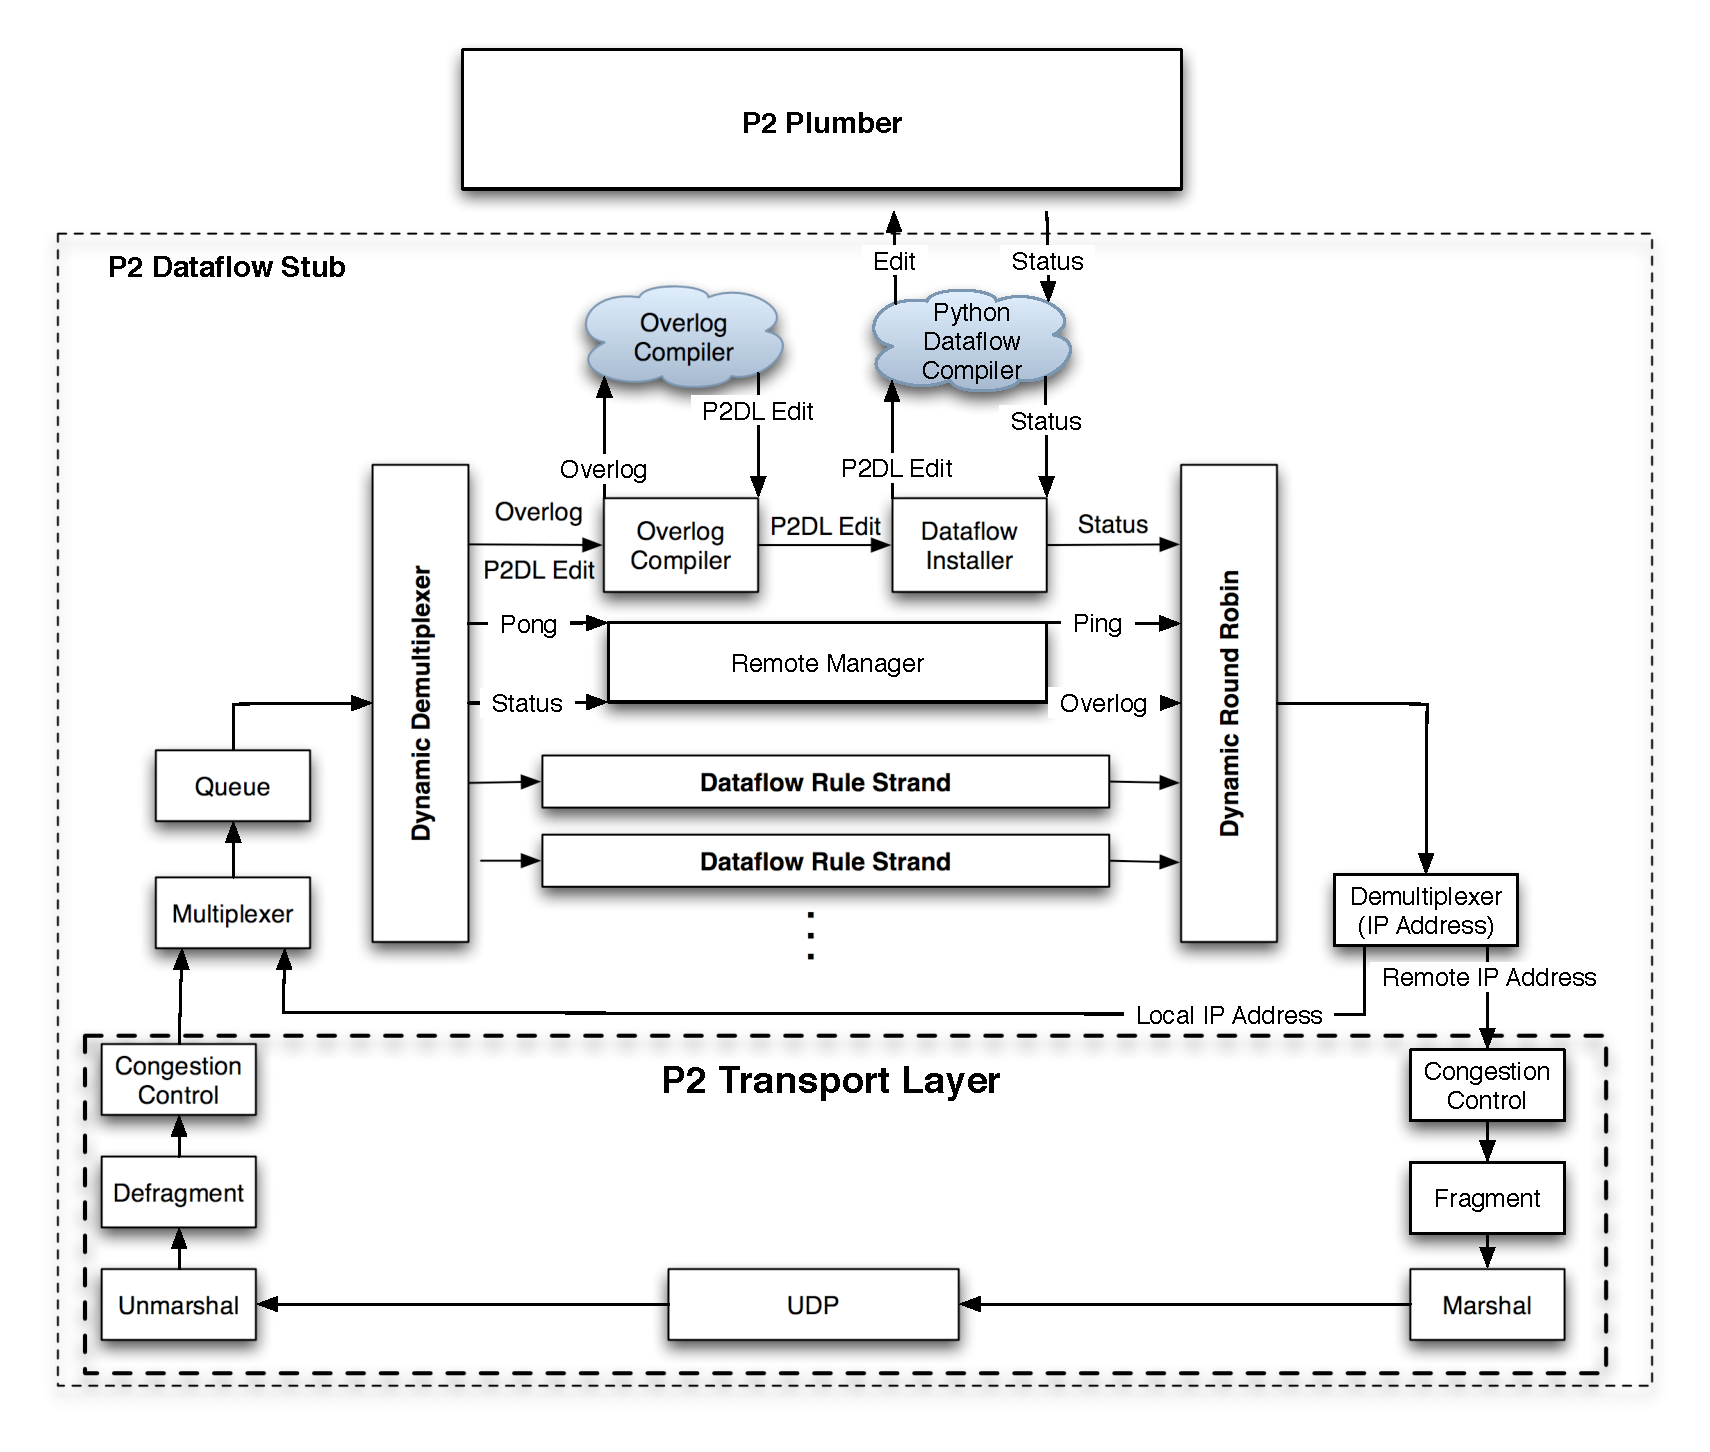
\includegraphics[width=6in]{p2stub.eps} 
   \caption{P2 stub node.}
   \label{fig:p2stub}
\end{figure*}

To incrementally install a set of OverLog rules into a running Plumber a node must have
installed the dataflow depicted in Figure~\ref{fig:p2stub}. The stub dataflow defines a transport layer
for receiving tuple data out of P2 network elements. The tuples received by a P2 stub node
can contain OverLog rules, a P2 dataflow edit script, Remote Manager messages,
or data destined for some installed rule. Edits are permitted on the transport layer itself but only
through a dataflow edit written in P2DL. The baseline transport layer defines congestion control and fragmentation functionality. The fragmentation support permits the sending of arbitrarily long 
OverLog programs to a node. It is also possible to install other transport layer features (e.g., reliable delivery,
order delivery, etc.) by either editing the Python script that generates the stub or by
sending an appropriate P2DL edit. 

The rules of an OverLog program are compiled into a set of dataflow strands~\cite{p2:sosp} 
and dynamically installed into the dynamic demux and dynamic round robin elements. 
The default port (port 0) of the dynamic demux handles tuples that contain programs written 
in either OverLog or P2DL. A tuple containing an OverLog program is compiled by the 
OverlogCompiler element, which performs a call to the OverLog planner. The OverLog planner is 
equipped to generate a P2DL script, rather than performing the actual installation. This generated 
scripted is repackaged in a tuple and forwarded to the DataflowInstaller. The DataflowInstaller 
accepts tuples containing P2DL edits, provided by the OverlogCompiler or from some outside 
source~\footnote{The OverlogCompiler will simply pass any tuple containing a P2DL program to its 
output port.}. On receipt of a P2DL edit, the DataflowInstaller compiles the script using the P2DL 
Python compiler, which returns a \emph{Plumber::DataflowEdit} object. The DataflowInstaller 
installs the returned \emph{Plumber::DataflowEdit} object into the running Plumber. The status of this 
installation is tracked at every step and returned to the source.

\subsection{Terminal Source}
\label{sec:terminal}

Section~\ref{sec:element_example} described a \emph{Terminal} element, written entirely
in Python, for packaging input from {\bf stdin} in a tuple. We have extended this example
element to accept input in the form of an OverLog program, and send the program in a tuple
to a P2 stub node. The element takes care of packaging a program in the proper tuple format
and reporting the status of the installation returned by the stub node. A Remote Manager is
built into the P2 stub in order to compliment the Terminal process of disseminating an OverLog
program into a population. The Remote Manager and the process of setting up a dissemination
tree is further described in Section~\ref{sec:rm}. Given such a dissemination tree, the Terminal
element need only inject the OverLog program in the root of the tree in order for the program
to be completely installed in a population. Other installation strategies are possible, including
the installation of OverLog rules in a subset of the population.

\subsection{Remote Manager}
\label{sec:rm}

\subsubsection{Overview}
Running a P2 program on a large collection of nodes requires a system for initially starting
up the program and recovering from node failures, which are common in real world deployments. 
To this end, a Remote Manager P2 element was written to 
start P2 stubs on other machines and monitor those machines, restarting the stubs when the 
machines fail or reboot.  The Remote Manager element was written in Python using the P2 Python 
library.

\subsubsection{Implementation}

The Remote Manager element is used to establish and maintain a default distribution tree 
for OverLog code installation into a group of nodes.  One node is selected as the 
root node and is seeded with a list of hosts to receive the initial program and any 
subsequent updates.  The root node removes
several machines from the beginning of the host list and designates them as its children.
It then sends a special ``ping'' message to those children to see if they are alive and 
participating in the distribution
tree (which, initially, they are not).  When a parent does not hear from one of its children,
it restarts the child by connecting to the remote machine and starting a stub P2 node script 
that contains a Remote Manager element, and provides that Remote Manager element with a 
list of nodes in that child's subtree.  The child then selects its children from the list 
and the process repeats.  Restarting a node takes a significant amount of time (seconds), 
during which the single-threaded P2 engine would drop incoming packets.  Python implements
threading, but it is user-level threading, which does not work well with the non-yielding 
C++ P2 engine.  To solve this, a separate process is forked whenever a node is re-started.


Periodically a node pings its children.  When a child is running, it responds with a ``pong''
that includes the number of P2 rules it has received from its parent.  If the parent has 
rules that the child has not seen, it sends the first unseen rule; this occurs both when 
new code is distributed and when a failed node is restarted.  The rule goes directly 
to the child's OverLog Compiler element which, in addition to sending the compiled script 
to the Dataflow Installer 
element, also sends all OverLog rules, in its log, to the child's Remote Manager element.  The 
Remote Manager maintains a sequential log of all of these rules from the OverLog Compiler.
When a child's Remote Manager sends a pong to its parent, it includes the current length 
of its OverLog rule log.

To speed recovery after failure, when a child receives a new rule, it sends an unsolicited 
pong with the new length of its
OverLog rule log.  If additional rules are waiting for the child, the parent will detect this
when it processes the pong and send the next rule.

If a parent does not hear from its child due to network effects (the ping or pong was lost),
then the parent will erroneously try to restart the P2 stub; however, this will harmlessly 
fail since 
the new P2 stub will try to open a pre-established port number which is already owned by the 
currently running P2 stub process and the new P2 stub will exit.

\eat {
\subsection{Experimental Results}

\begin{figure*}[htbp] %  figure placement: here, top, bottom, or page
   \centering
   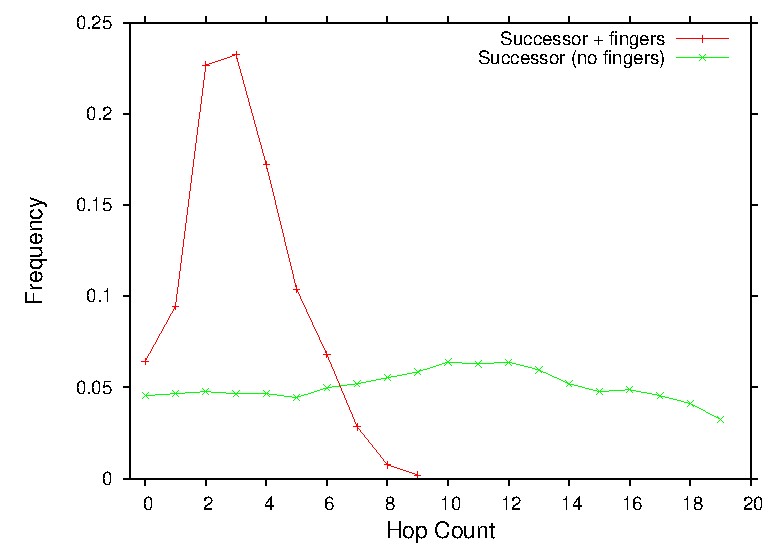
\includegraphics{./data/hop_lookup.eps} 
   \caption{Hop count frequency.}
   \label{fig:hop_freq}
\end{figure*}

In this section we describe some results obtained by running a set of P2 nodes on
a machine equipped with $7$ $2.0$ GHz Xeon processors. All experiments contain
a population of $21$ P2 nodes that are initialized with the P2 Python stub script described
in Section~\ref{sec:p2stub}. We are working toward experimental results from a more realistic environment such as PlanetLab~\cite{planetlab}. However, due to time limitations such results could
not be obtained for this version of the write-up. We note that the status of the code is ready for
such a deployment, and it will occur in the very near future. 

The set of experiments described in this section deal with deploying the P2 nodes and
incrementally installing the OverLog rules for a Chord overlay network~\cite{p2:sosp},
\cite{chord}. Figure~\ref{fig:hop_freq} presents results from two Chord experiments. 
The first experiment installs the full version of Chord, including rules for establishing
successors (the base Chord ring) and a full arsenal of finger entries (nodes at powers
of 2 away from the origin node identifier). The second experiment omits the rules for
establishing finger entries, leaving only the successor rules for creating the basic Chord 
ring overlay. After all nodes reconcile their state for finger and successor entries, we begin
issuing lookups for random identifiers, originating from a predefined set of 5 nodes~\footnote{We
check that the ring and finger entries are properly formed before injecting any lookup tuples.}. 

\begin{figure*}[htbp] %  figure placement: here, top, bottom, or page
   \centering
   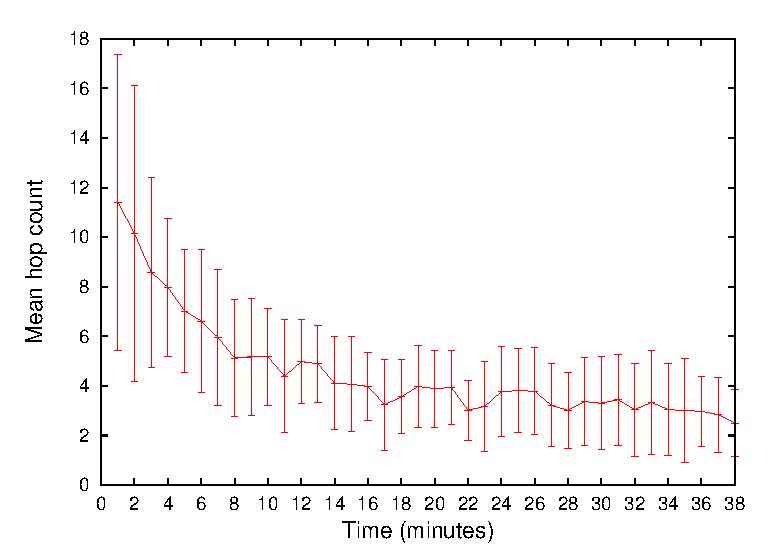
\includegraphics{./data/hop_lookup_dynamic.eps} 
   \caption{Mean hop count during dynamic finger installation.}
   \label{fig:hop_dynamic}
\end{figure*}

The experiment measures the number of hops that each message takes on its way to 
the destination and plots the frequency along the y-axis of the corresponding hop count 
indicated along the x-axis. A hop count of $0$ indicates that the lookup is destined for the
node at which the lookup originates, while further hop counts travel through the overlay along
the indicated number of node hops. The graph shows what one would expect when nodes
are equipped with and without finger entries. The plot with fingers shows most lookup messages
taking around 2-3 hops, which is what one would expect ($\frac{1}{2}\log{21}$) from a stable 
Chord network. The plot without fingers shows most lookup messages traveling around 9-13 
hops, which is again the number of expected hops ($\frac{21}{2}$) that a message should take
in a baseline Chord ring overlay.

In our next, and final, experiment we install the rules for fingers into the nodes of a Chord network primed with
successors (installed by successor rules), all the while measuring hop counts from randomly 
generated lookup messages. The experiment begins
by installing, in all nodes, the (successor) rules that form the base Chord ring. We logically 
divide the nodes into $4$ groups, three of which contain $5$ nodes and the last having 
$6$ nodes. A node from each group is selected as the origin of a lookup message, destined 
for a random identifier. A lookup message is generated and sent to each designated node
every 5 seconds. That is, four random lookups are injected into the population every 5 seconds. 
The lookup message generator waits until all nodes in the overlay network discover their true successor, which occurs at $Time=0$ along Figure~\ref{fig:hop_dynamic}. At $Time=1$ minute we install the finger
rules into the first group of $5$ nodes. We continue this process by installing finger rules into 
the other $3$ node groups at times $3$, $5$, and $7$ minutes. The lookup generator continually 
injects random lookups while the finger rules are being distributed and installed.

The graph shown in Figure~\ref{fig:hop_dynamic} plots the mean and stddev hop count of 
the randomly generated lookup message, over time, during the process of finger installation. 
As mentioned above, finger installation begins at $Time=0$ and ends at $Time=7$ minutes.
The graph shows the mean hop count decreasing as finger rules are installed into the population.
The benefits of fingers are shown by this reduction in the mean hop count.
 }

\bibliography{paper}
\end{document}